\begin{pastexam}[label={px:gk3-108-ds-04}]{高考三級資訊處理 108 年 第四題}
（申論；25 分）

用 $G = (V, E)$ 表示一個無方向性圖形，其中 $V$ 是點的集合，$E$ 是一組節點（Vertices）形成一個邊及對應
權重（Weights）所組成的集合，例如：$(0, 1, 28)$ 表示節點 $0$ 至節點 $1$ 有一個邊，而且權重為 $28$。今有一
圖形 $G = (V, E)$，$V = \{0, 1, 2, 3, 4, 5, 6\}$，$E = \{(0, 1, 27), (1, 2, 15), (2, 3, 11), (0, 5, 9),
(1, 6, 13), (4, 5, 24), (4, 6, 23), (3, 4, 21), (3, 6, 17)\}$。請利用 Kruskal 演算法計算最小擴張樹
（Minimum spanning tree）之最低權重或成本值。（25 分）
\end{pastexam}

\begin{pastsoln}
答案：$93$（邊 $(0,5)$、$(2,3)$、$(1,6)$、$(1,2)$、$(3,4)$、$(4,5)$）。

\textbf{做法}（資結書第~24.2~節、虛擬碼~24.2）：把邊依權重由小到大排，依序檢查；兩端點在不同的連通塊
（用互斥集合判斷）就收進來並合併兩塊，同一塊就會形成迴路，丟掉。 收滿 $|V| - 1 = 6$ 條就停。
\begin{center}
\begin{tabular}{cccl}
\toprule
順序 & 邊 & 權重 & 結果與收邊後的連通塊 \\
\midrule
1 & $(0,5)$ & 9 & 收；$\{0,5\}$ \\
2 & $(2,3)$ & 11 & 收；$\{0,5\}$、$\{2,3\}$ \\
3 & $(1,6)$ & 13 & 收；$\{0,5\}$、$\{2,3\}$、$\{1,6\}$ \\
4 & $(1,2)$ & 15 & 收；$\{0,5\}$、$\{1,2,3,6\}$ \\
5 & $(3,6)$ & 17 & 丟：$3$、$6$ 已在同一塊（$3$--$2$--$1$--$6$），會成迴路 \\
6 & $(3,4)$ & 21 & 收；$\{0,5\}$、$\{1,2,3,4,6\}$ \\
7 & $(4,6)$ & 23 & 丟：$4$、$6$ 已在同一塊 \\
8 & $(4,5)$ & 24 & 收；$\{0,1,2,3,4,5,6\}$，已有 $6$ 條邊，結束 \\
\bottomrule
\end{tabular}
\end{center}
$(0,1,27)$ 不用再看（就算看也會形成迴路）。 最小擴張樹的成本是
\[
9 + 11 + 13 + 15 + 21 + 24 = 93.
\]
\begin{center}
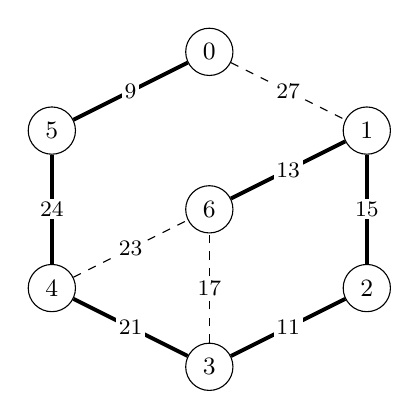
\begin{tikzpicture}[v/.style={circle,draw,minimum size=6mm,inner sep=0pt,font=\small},
  lab/.style={font=\footnotesize,fill=white,inner sep=1pt}, t/.style={line width=1.4pt}, n/.style={dashed}]
\node[v] (0) at (0,2) {0};
\node[v] (1) at (2,1) {1};
\node[v] (5) at (-2,1) {5};
\node[v] (6) at (0,0) {6};
\node[v] (2) at (2,-1) {2};
\node[v] (4) at (-2,-1) {4};
\node[v] (3) at (0,-2) {3};
\draw[n] (0) -- node[lab] {27} (1);
\draw[t] (0) -- node[lab] {9} (5);
\draw[t] (1) -- node[lab] {13} (6);
\draw[t] (1) -- node[lab] {15} (2);
\draw[t] (2) -- node[lab] {11} (3);
\draw[t] (4) -- node[lab] {24} (5);
\draw[n] (4) -- node[lab] {23} (6);
\draw[t] (3) -- node[lab] {21} (4);
\draw[n] (3) -- node[lab] {17} (6);
\end{tikzpicture}
\end{center}
粗線是最小擴張樹，虛線是沒選的邊。 所有權重都不同，所以最小擴張樹唯一（資結書定理~24.4）。
\end{pastsoln}
